\documentclass{article}

\usepackage{ssArxiv}

\usepackage[utf8]{inputenc}

\usepackage[title]{appendix}

\usepackage{amsmath,amsbsy,amsgen,amscd,amssymb,amsthm,amsfonts}
\usepackage{mathtools}
\usepackage{booktabs}
\usepackage{bm}
\usepackage{enumitem}
\usepackage{subcaption, geometry, graphicx, lipsum}
\usepackage{microtype}
\usepackage{multirow}
\usepackage[
  pagebackref=true,
  colorlinks=true,
  citecolor=MidnightBlue,
  linkcolor=Fuchsia,
]{hyperref}
\usepackage{pifont}
\usepackage[nameinlink]{cleveref}
\usepackage{url} 
\usepackage{graphicx}
\usepackage{algorithm,algorithmic}
\usepackage{natbib}
\usepackage{xspace}
\usepackage{caption}
\captionsetup[table]{skip=5pt}
\usepackage{listings}
\lstset{
  basicstyle=\ttfamily\footnotesize,
  columns=fullflexible,
  frame=single,
  breaklines=true,
  postbreak=\mbox{$\hookrightarrow$\space},
  rulecolor=\color{black},
}
\lstset{moredelim=[is][\color{red}]{!*}{*!}} 

\definecolor{codegreen}{rgb}{0,0.6,0}
\lstdefinestyle{mystyle}{  
    commentstyle=\color{codegreen},
    keywordstyle=\color{blue},
    basicstyle=\ttfamily\footnotesize,
    breakatwhitespace=false,         
    breaklines=true,                 
    captionpos=b,                    
    keepspaces=true,                 
    showspaces=false,                
    showstringspaces=false,
    showtabs=false,                  
    tabsize=2
}
\lstset{style=mystyle}

\usepackage[dvipsnames]{xcolor}
\usepackage[most]{tcolorbox}

% Define the color
\definecolor{lightgreen}{HTML}{C4FFCF}

\newtheorem{lemma}{Lemma}
\newtheorem{corollary}{Corollary}
\newtheorem{remark}{Remark}
\newtheorem{theorem}{Theorem}
\newtheorem{assumption}{Assumption}
\crefname{assumption}{assumption}{assumptions}
\newtheorem{definition}{Definition}

\newcommand{\red}[1]{\textbf{\textcolor{red}{#1}}}
\newcommand{\green}[1]{\textbf{\textcolor{ForestGreen}{#1}}}

\newcommand{\cmark}{\ding{51}}
\newcommand{\xmark}{\ding{55}}
\newcommand{\benchmark}{\textsc{CRUXEval}\xspace}
\newcommand{\benchmarki}{\textsc{CRUXEval-I}\xspace}
\newcommand{\benchmarko}{\textsc{CRUXEval-O}\xspace}

\newcommand{\codellamamed}{\textsc{Code Llama 13B}\xspace}
\newcommand{\codellamalarge}{\textsc{Code Llama 34B}\xspace}

\makeatletter
\newcommand\nnfootnote[1]{%
  \begin{NoHyper}
  \renewcommand\thefootnote{}\footnote{#1}%
  \addtocounter{footnote}{-1}%
  \end{NoHyper}
}

\makeatother
  
\setlength{\parindent}{0em}
\setlength{\parskip}{0.75em}


\renewcommand*\backref[1]{\ifx#1\relax \else (Cited on pg. #1) \fi}
% Measuring code grounding through predicting execution
% Measuring execution ability of code models
% Execution Benchmark
% World models of code models
\title{CRUXEval: A Benchmark for Code Reasoning, Understanding and Execution \\ \ \newline \large \href{https://crux-eval.github.io/}{www.crux-eval.github.io}}
\author{\name Alex Gu$^{\star}$
\email{gua@mit.edu} \\
\addr{MIT CSAIL} \\
\name Baptiste Rozière
\email{broz@meta.com} \\
\addr{Meta AI} \\
\name Hugh Leather
\email{hleather@meta.com} \\
\addr{Meta AI} \\
\name Armando Solar-Lezama
\email{asolar@csail.mit.edu} \\
\addr{MIT CSAIL} \\
\name Gabriel Synnaeve
\email{gab@meta.com} \\
\addr{Meta AI} \\
\name Sida I. Wang
\email{sida@meta.com} \\
\addr{Meta AI} \\
}

\makeatletter
\let\c@table\c@figure % for (1)
\let\ftype@table\ftype@figure % for (2)
\makeatother

\begin{document}
\begin{figure}[H]
    \centering
    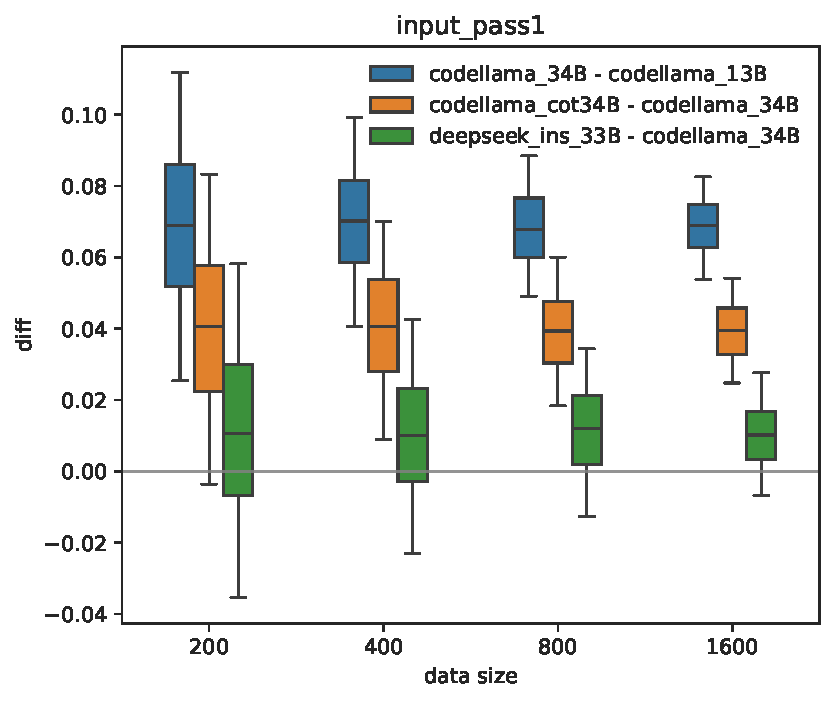
\includegraphics[width=0.49\textwidth] {figs/wrong_order/wrong_order_box_input_pass1.pdf}
    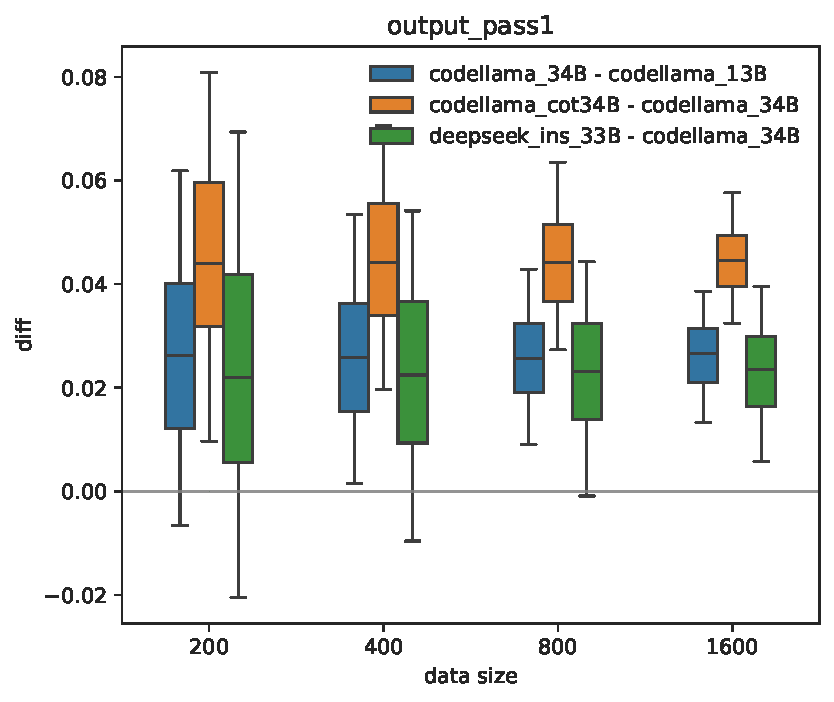
\includegraphics[width=0.49\textwidth]{figs/wrong_order/wrong_order_box_output_pass1.pdf}
    \caption{Probability of mis-sorting $\codellamamed$ and $\codellamalarge$ on bootstrap samples of various sizes. The whiskers show (2.5, 97.5) and boxes show (25, 75) percentiles. }
    \label{fig:benchmark-filtering-size-selection}
\end{figure}

\begin{figure}[H]
     \centering
     \begin{subfigure}[b]{0.49\textwidth}
         \centering
         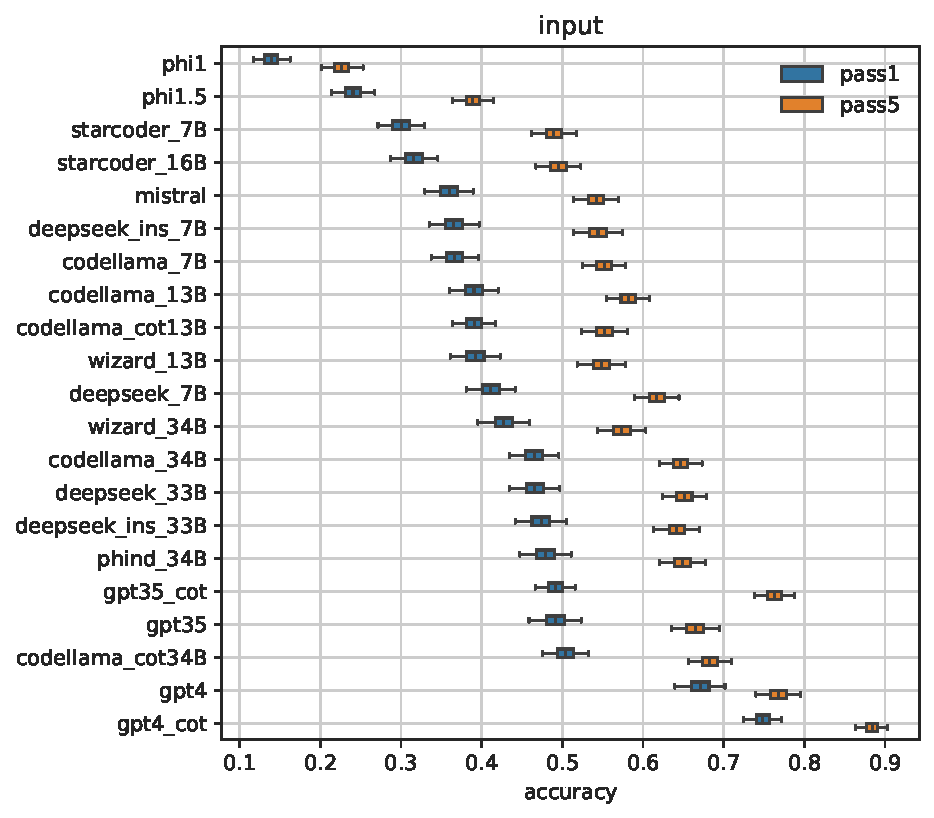
\includegraphics[width=\textwidth]{figs/main_results/main_box_input.pdf}
         \caption{\benchmarki Performance}
         \label{fig:main-results-pass1-input}
     \end{subfigure}
     \hfill
     \begin{subfigure}[b]{0.49\textwidth}
         \centering
         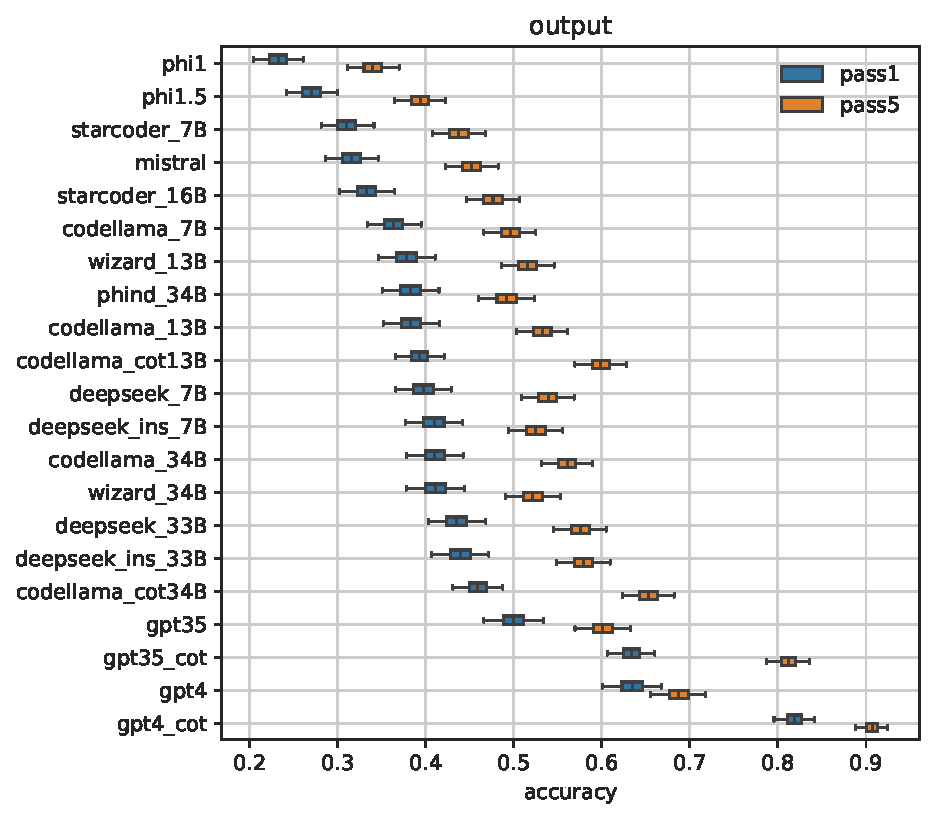
\includegraphics[width=\textwidth]{figs/main_results/main_box_output.pdf}
         \caption{\benchmarko Performance}
         \label{fig:main-results-pass1-output}
     \end{subfigure}
     \caption{Main Results. Boxes show (25, 75) percentiles, whiskers show (2.5, 97.5), and the middle bar shows the median ($\approx$ mean). }
     \label{fig:main-results}
\end{figure}

\begin{table}[htbp]
    \centering
    \caption{Impact of Anonymization on \benchmark}
    \begin{tabular}{cccccc}
        \toprule
        \textbf{Model} & \textbf{Anonymized} & \textbf{Input Pass@1} & \textbf{Output Pass@1} \\
        \midrule
        \multirow{3}{*}{CodeLlama 7B} 
	& \xmark & 36.6\% & 36.4\% \\
        & \cmark & 37.5\% & 34.0\% \\
        & $\Delta$ & \green{+0.9\%} & \red{-2.4\%} \\
        \midrule
        \multirow{3}{*}{CodeLlama 13B} 
        & \xmark & 39.0\% & 38.3\%  \\
        & \cmark & 40.0\% & 36.1\% \\
        & $\Delta$ & \green{+1.0\%} & \red{-2.2\%} \\
        \midrule
        \multirow{3}{*}{CodeLlama 34B} 
        & \xmark & 46.5\% & 41.1\% \\
        & \cmark & 48.0\% & 39.1\% \\
        & $\Delta$ & \green{+1.5\%} & \red{-2.0\%} \\
        \bottomrule
    \end{tabular}
    \label{tab:benchmark-results-anonymous}
\end{table}

\begin{figure}[H]
     \centering
     \begin{subfigure}[b]{0.49\textwidth}
         \centering
         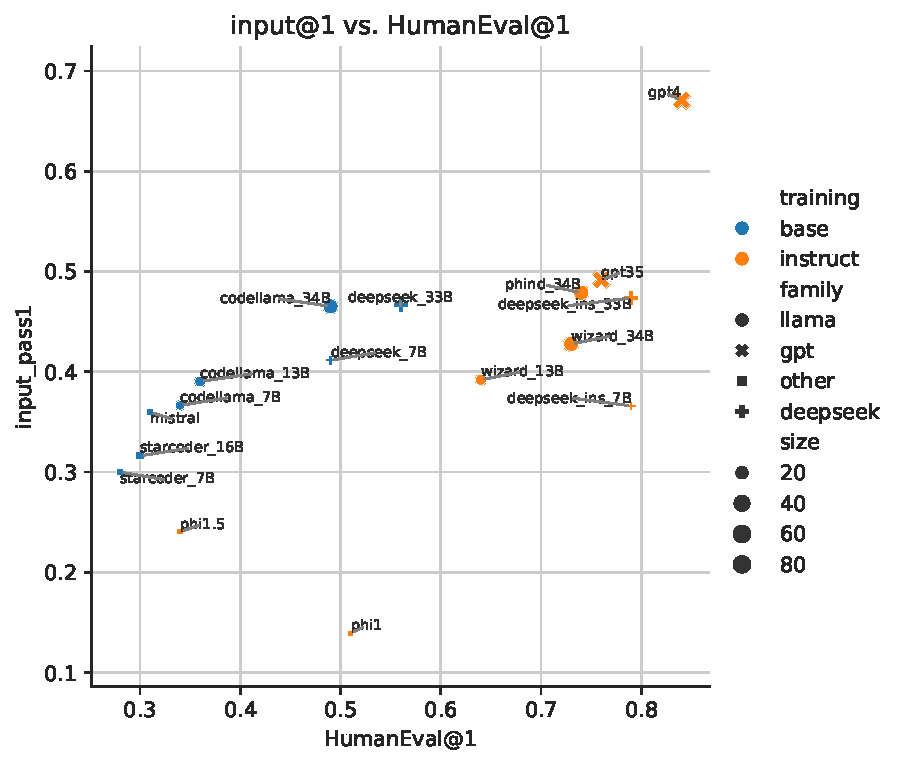
\includegraphics[scale=0.49]{figs/scatter/HumanEval_1_vs_input_pass1.pdf}
         \caption{\benchmarki vs. HumanEval}
         \label{fig:quant-analysis-humaneval-correlation-input}
     \end{subfigure}
     \hfill
     \begin{subfigure}[b]{0.49\textwidth}
         \centering
         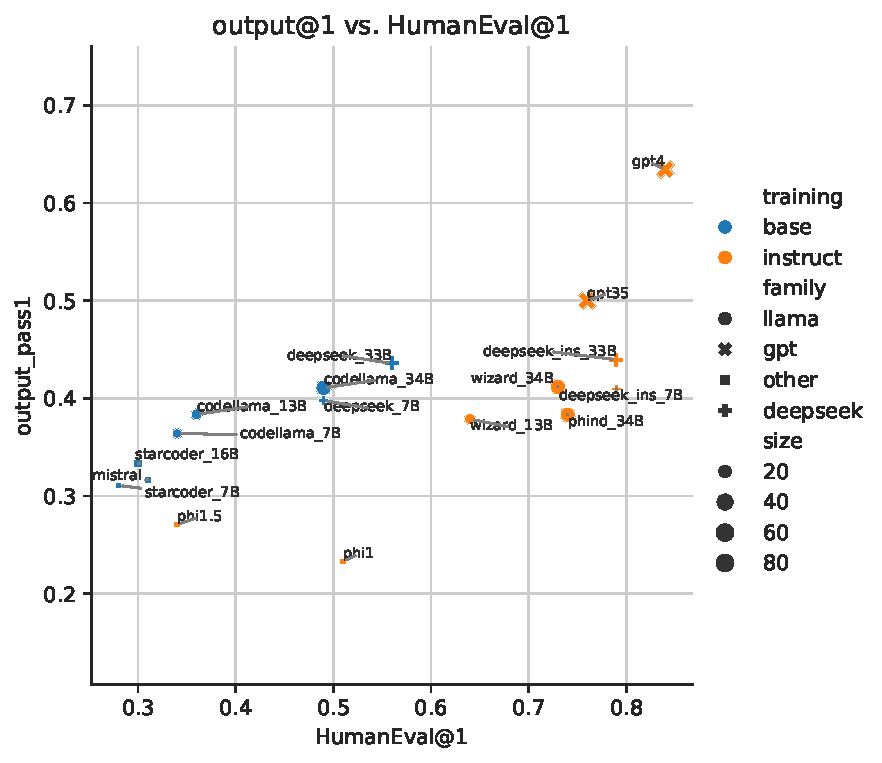
\includegraphics[scale=0.49]{figs/scatter/HumanEval_1_vs_output_pass1.pdf}
         \caption{\benchmarko vs. HumanEval}
         \label{fig:quant-analysis-humaneval-correlation-output}
     \end{subfigure}
     \caption{Correlation between HumanEval pass@1 scores and \benchmarko pass@1 scores}
     \label{fig:quant-analysis-humaneval-correlation-1}
\end{figure}

\begin{figure}[H]
     \centering
     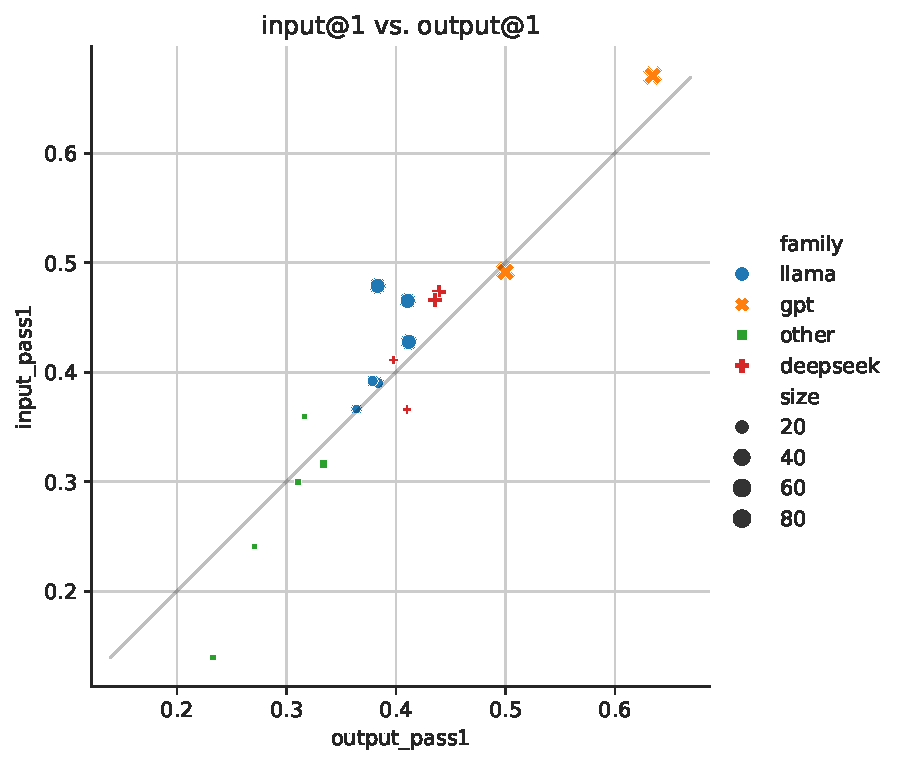
\includegraphics[scale=0.49]{figs/scatter/output_1_vs_input_1.pdf}
     \caption{Correlation between Input and Output Prediction Scores}
     \label{fig:quant-analysis-input-output}
\end{figure}

\begin{figure}[H]
     \centering
     \begin{subfigure}[b]{0.49\textwidth}
         \centering
         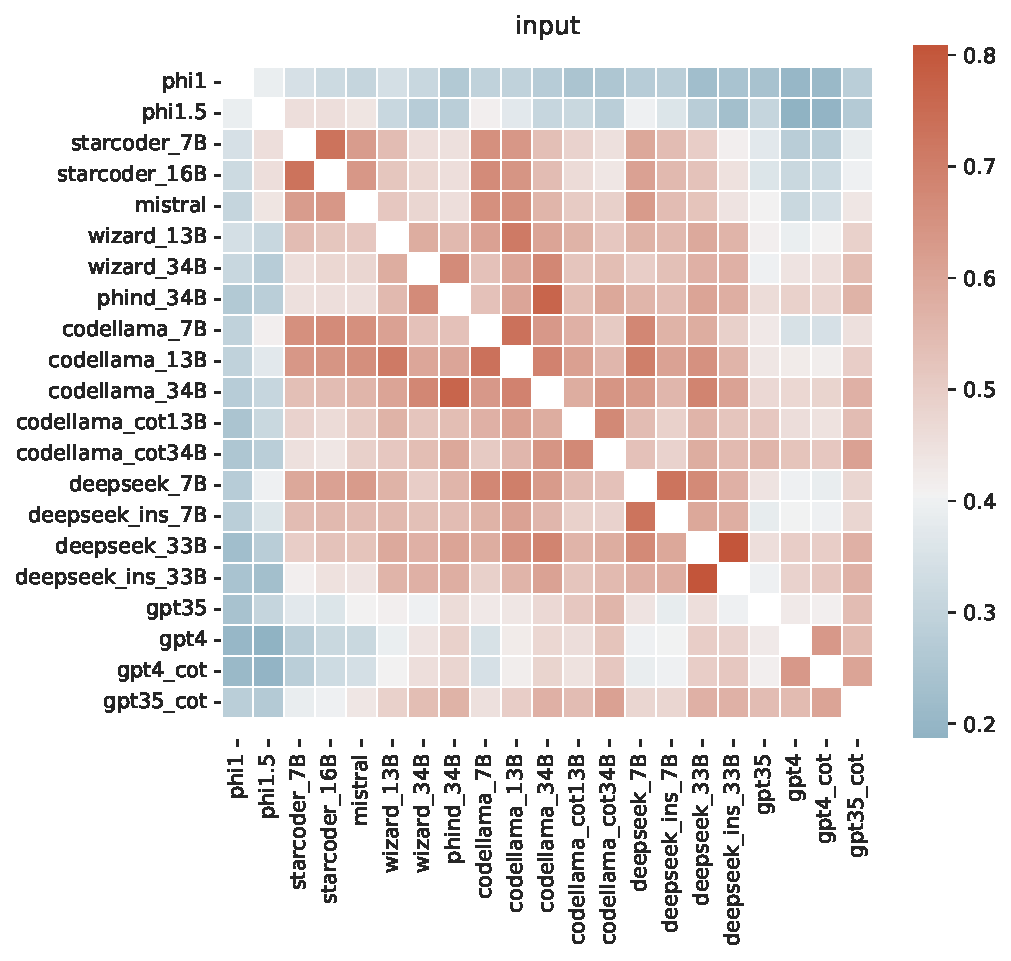
\includegraphics[width=1\textwidth]{figs/error_correlation_input_heatmap.pdf}
     \end{subfigure}
     \hfill
     \begin{subfigure}[b]{0.49\textwidth}
         \centering
         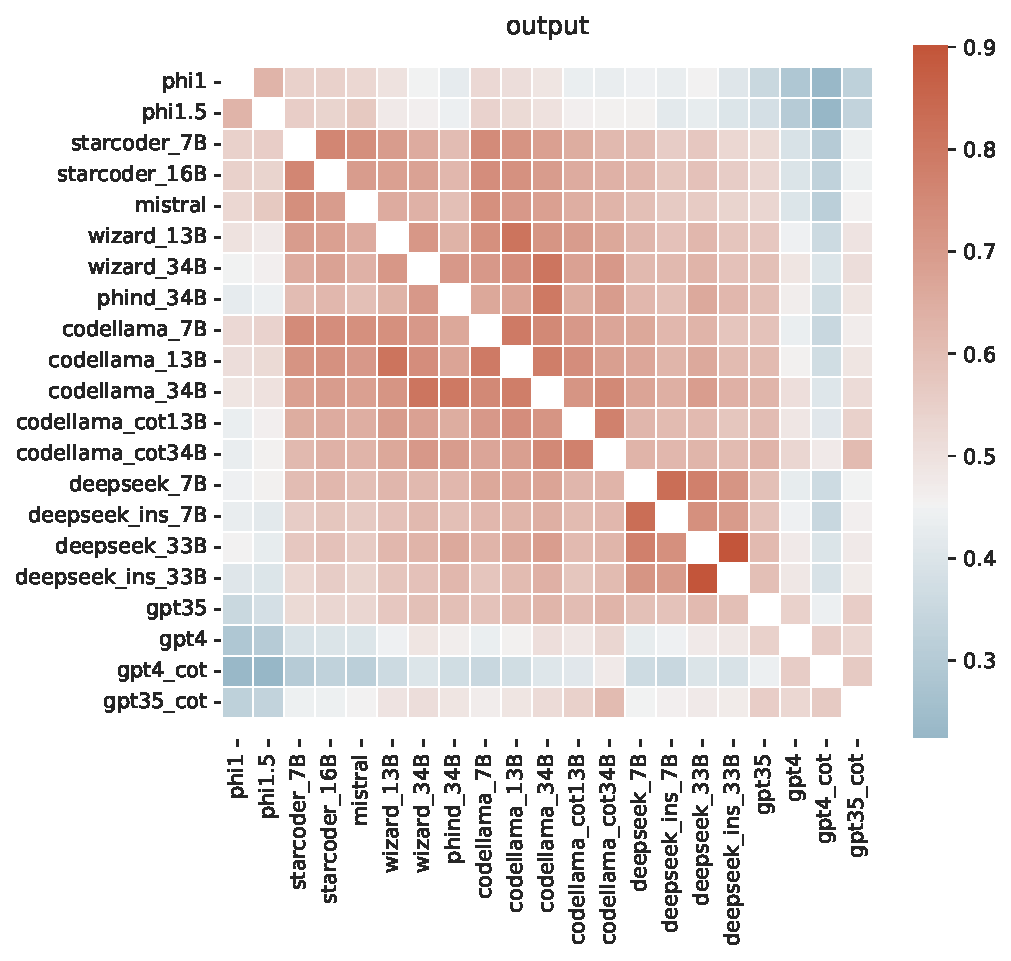
\includegraphics[width=1\textwidth]{figs/error_correlation_output_heatmap.pdf}
     \end{subfigure}
     \caption{Correlation between predictions on input (left) and output (right)}
     \label{fig:error_corr-input-output}
\end{figure}

\begin{figure}[H]
     \centering
     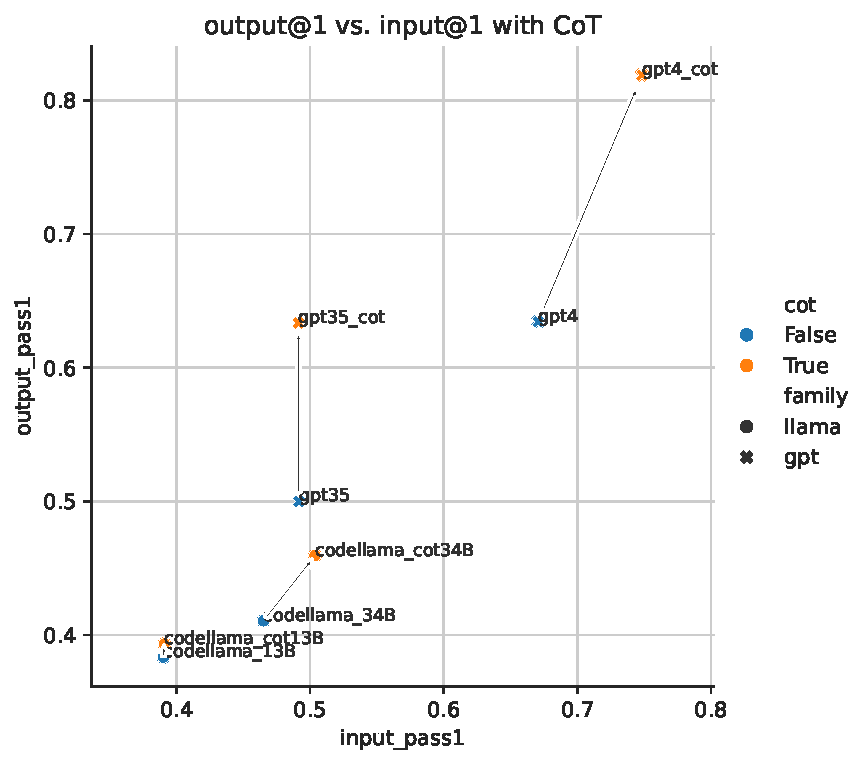
\includegraphics[scale=0.49]{figs/scatter/cot_input_pass1_output_pass1.pdf}
     \caption{Correlation between Input and Output Prediction Scores}
     \label{fig:quant-analysis-input-output}
\end{figure}


\begin{figure}[H]
     \centering
     \begin{subfigure}[b]{0.49\textwidth}
         \centering
         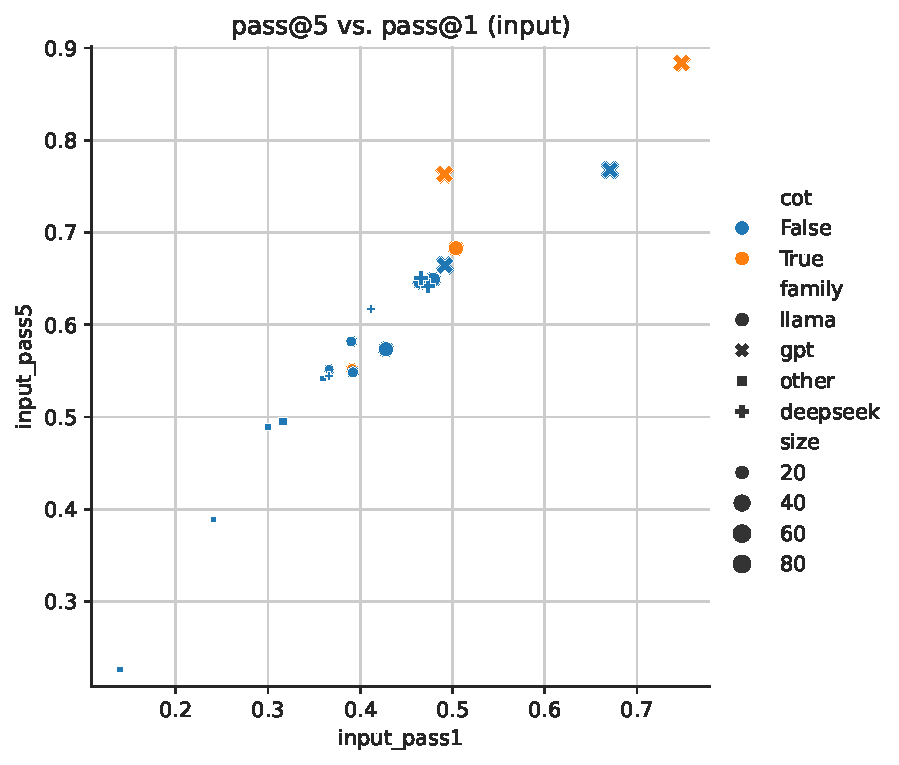
\includegraphics[scale=0.45]{figs/scatter/input_pass_5v1.pdf}
         \caption{Input prediction}
         \label{fig:pass5-vs-pass1-cot-input}
     \end{subfigure}
     \hfill
     \begin{subfigure}[b]{0.49\textwidth}
         \centering
         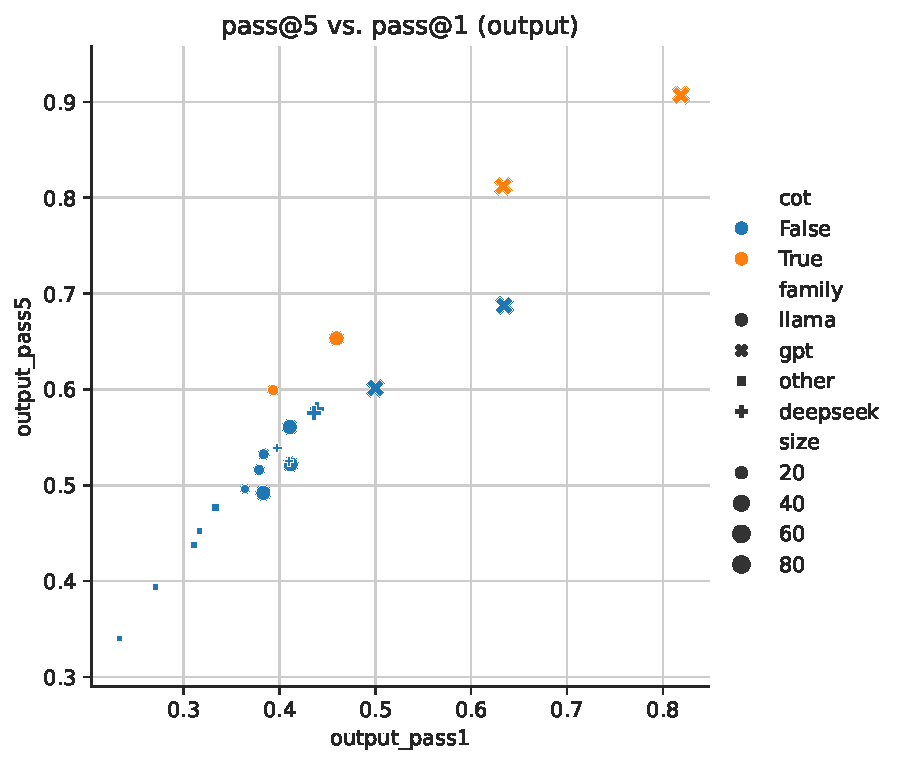
\includegraphics[scale=0.45]{figs/scatter/output_pass_5v1.pdf}
         \caption{Output prediction}
         \label{fig:pass5-vs-pass1-cot-output}
     \end{subfigure}
     \caption{pass@5 score vs. pass@1 score with and without CoT}
     \label{fig:pass5-vs-pass1-cot}
\end{figure}


\begin{figure}[H]
     \centering
     \begin{subfigure}[t]{0.49\textwidth}
         \centering
         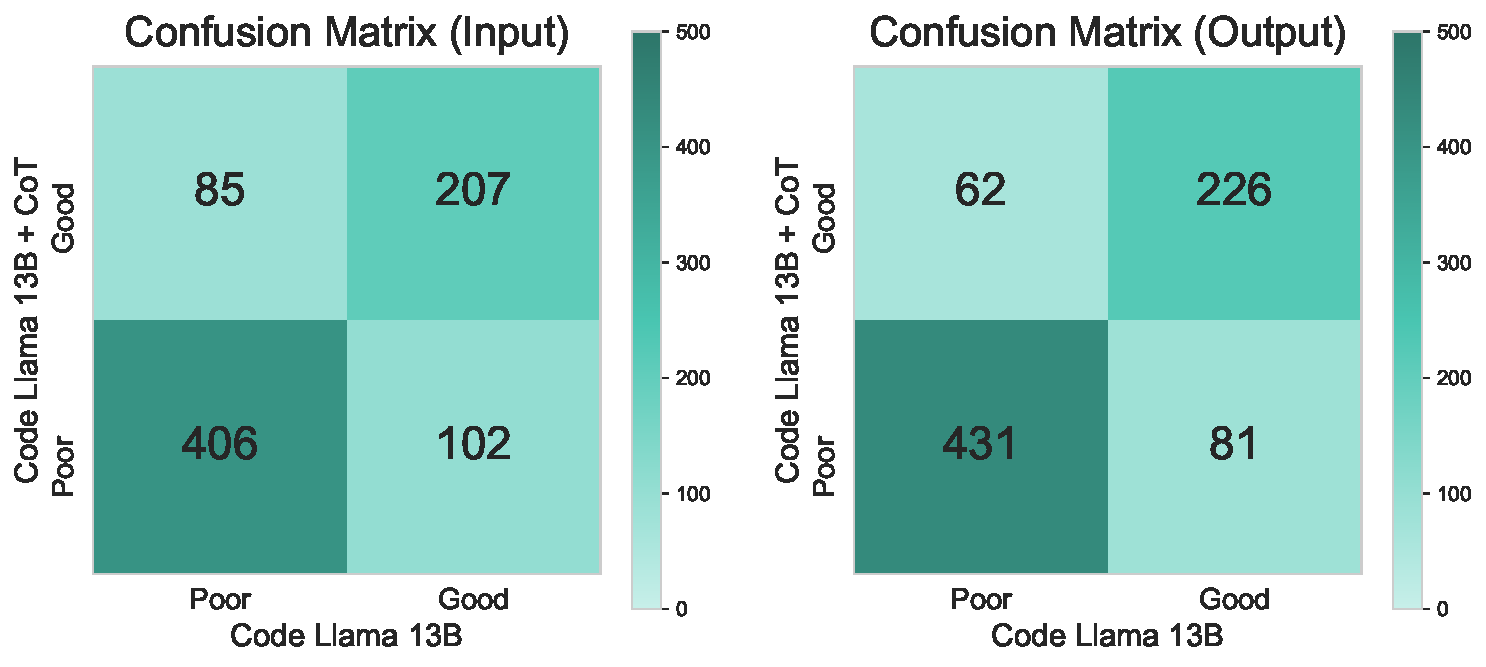
\includegraphics[width=\textwidth]{figs/confusion_cot_blogpost/confusion_codellama_13B_codellama_cot13B_blogpost.pdf}
         \caption{Code Llama 13B}
         \label{fig:confusion-cot-codellama-13b}
     \end{subfigure}%
     \hfill
     \begin{subfigure}[t]{0.49\textwidth}
         \centering
         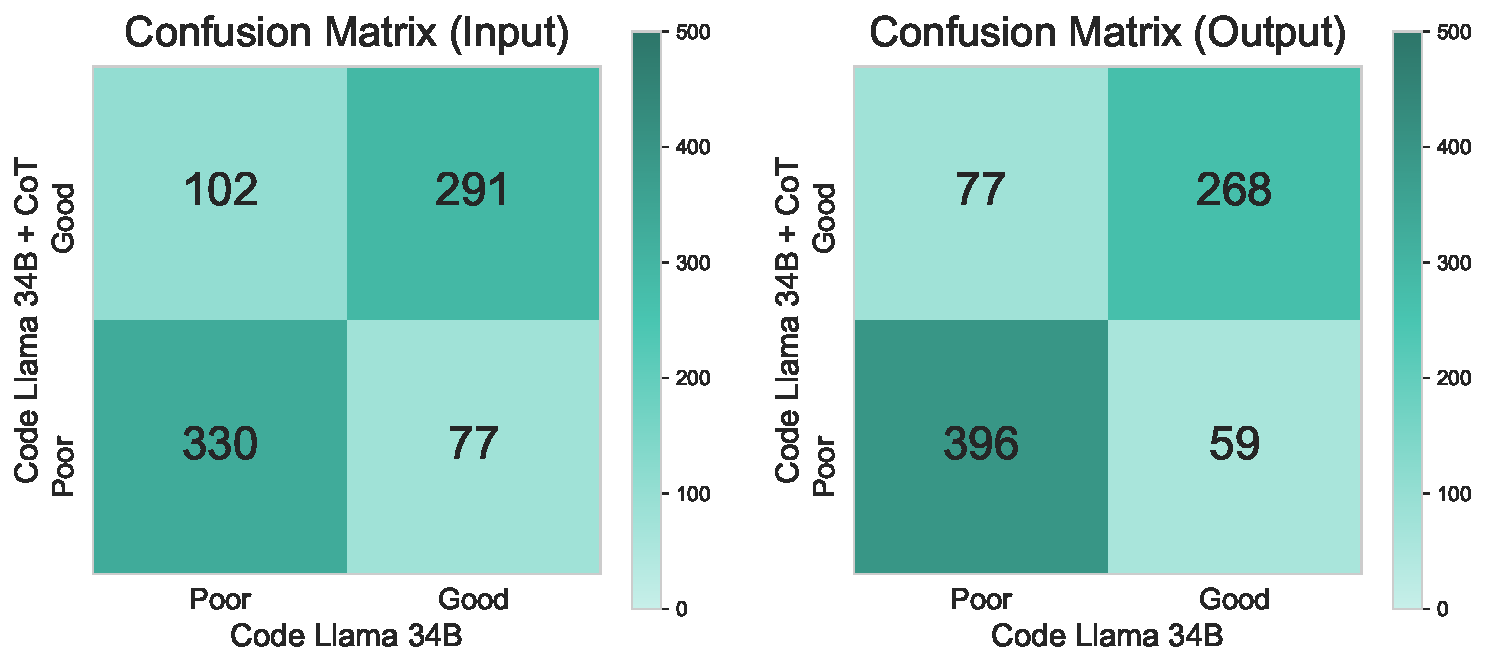
\includegraphics[width=\textwidth]{figs/confusion_cot_blogpost/confusion_codellama_30B_codellama_cot30B_blogpost.pdf}
         \caption{Code Llama 34B}
         \label{fig:confusion-cot-codellama-34b}
     \end{subfigure}
     \newline
     \newline
     \newline
     \begin{subfigure}[t]{0.49\textwidth}
         \centering
         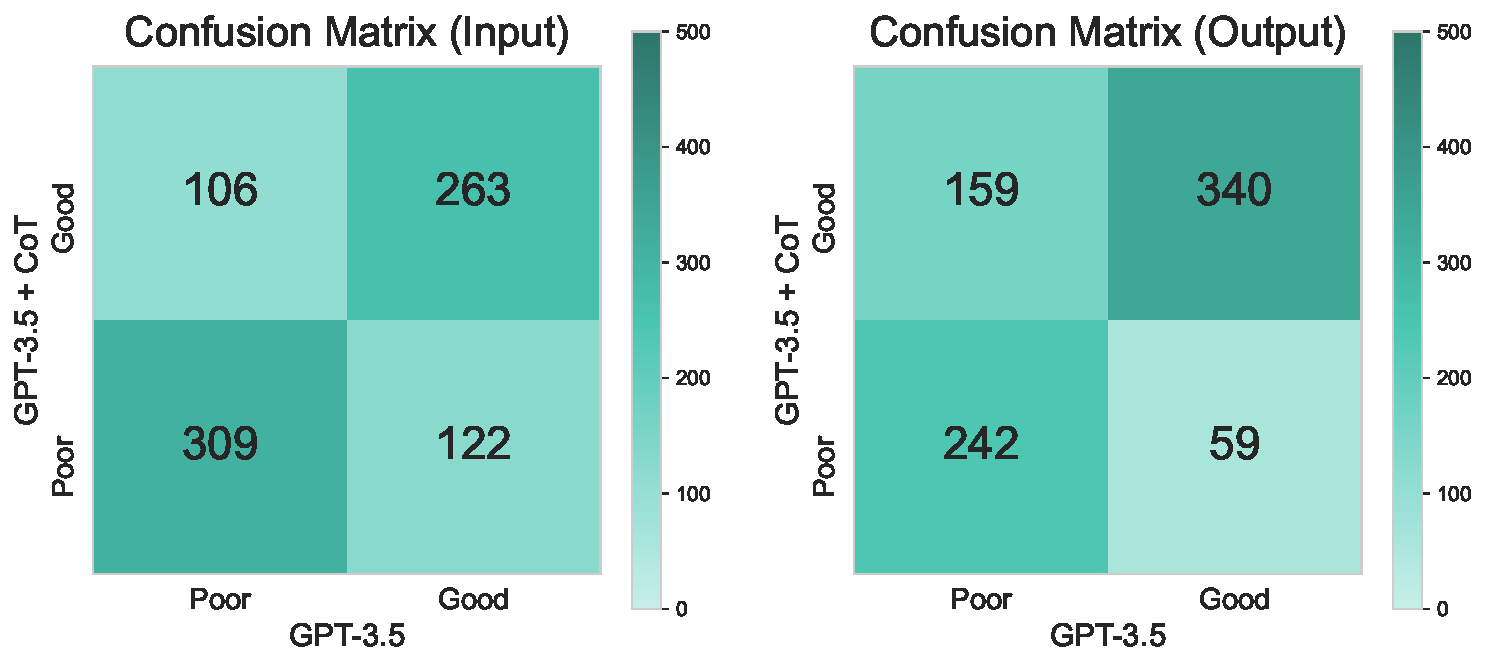
\includegraphics[width=\textwidth]{figs/confusion_cot_blogpost/confusion_gpt35_gpt35_cot_blogpost.pdf}
         \caption{GPT-3.5}
         \label{fig:confusion-cot-gpt35}
     \end{subfigure}%
     \hfill
     \begin{subfigure}[t]{0.49\textwidth}
         \centering
         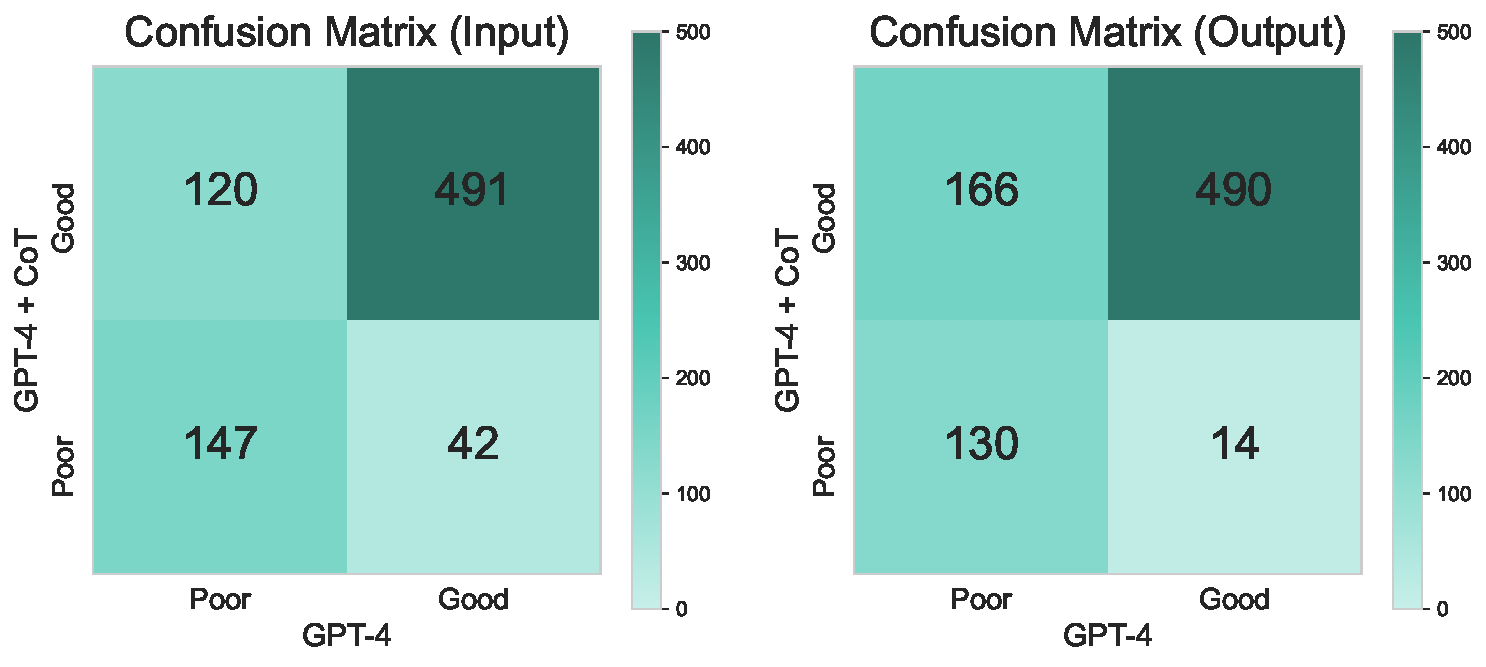
\includegraphics[width=\textwidth]{figs/confusion_cot_blogpost/confusion_gpt4_gpt4_cot_blogpost.pdf}
         \caption{GPT-4}
         \label{fig:confusion-cot-gpt4}
     \end{subfigure}
     \caption{Confusion Matrix of Direct Prediction vs. CoT Prediction $(T=0.2)$}
     \label{fig:confusion-cot-all}
\end{figure}

\begin{figure}[H]
     \centering
     \begin{subfigure}[b]{0.48\textwidth}
         \centering
         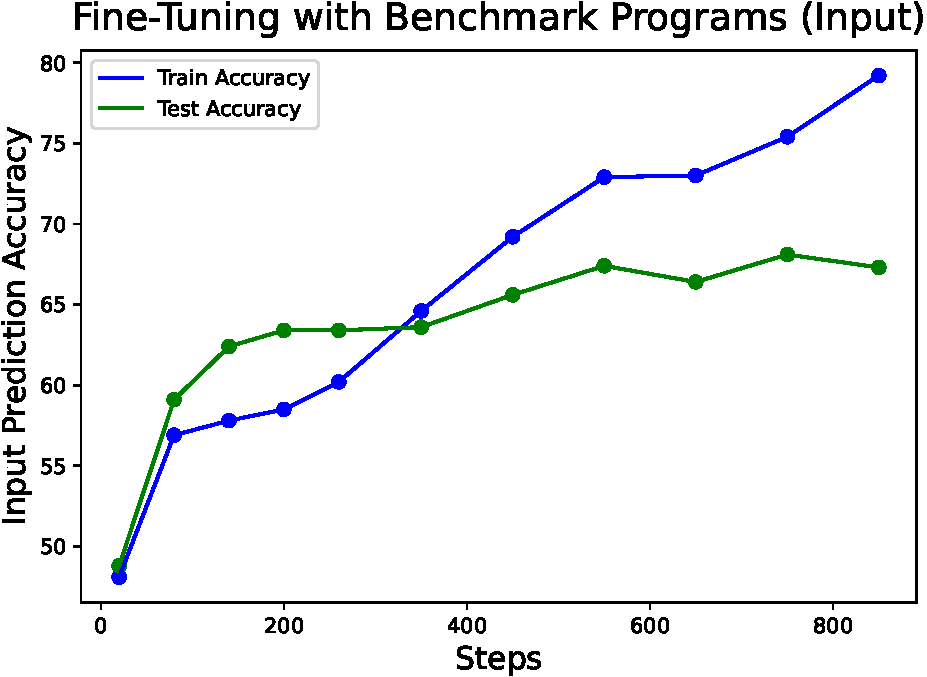
\includegraphics[scale=0.4]{figs/finetuning/finetuning_input_moredata_accuracy.pdf}
         \caption{Input prediction}
         \label{fig:finetuning-accuracy-samples-plot-input-main}
     \end{subfigure}
     \hfill
     \begin{subfigure}[b]{0.48\textwidth}
         \centering
         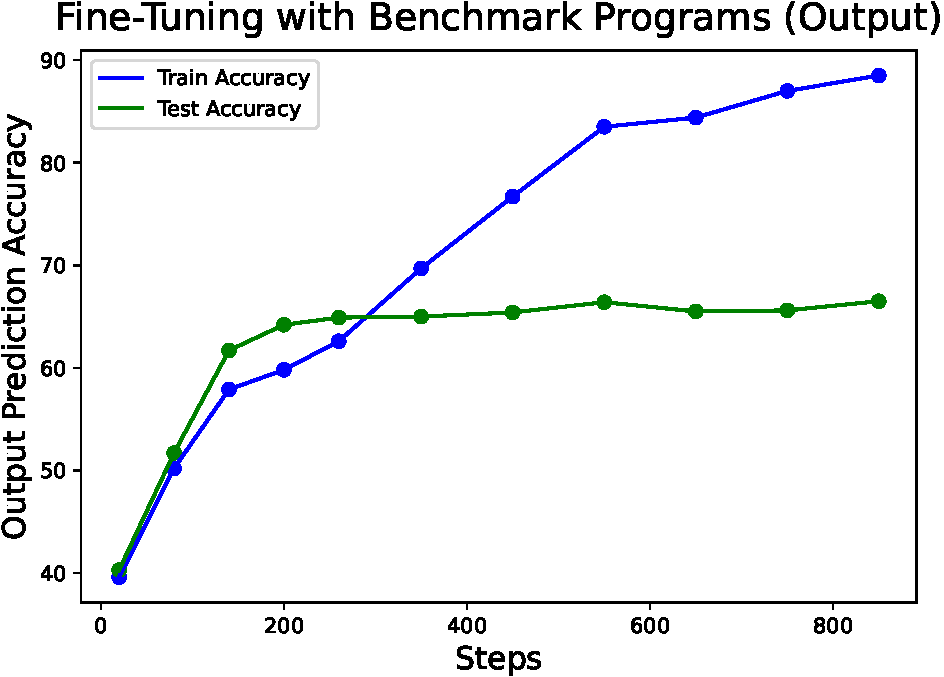
\includegraphics[scale=0.4]{figs/finetuning/finetuning_output_moredata_accuracy.pdf}
         \caption{Output prediction}
         \label{fig:finetuning-accuracy-samples-plot-output-main}
     \end{subfigure}
     \caption{Improvements and Limits of \benchmark Performance after Fine-Tuning}
     \label{fig:finetuning-accuracy-samples-plot-main}
\end{figure}

\begin{minipage}{.48\textwidth}
\begin{lstlisting}[label={lst:benchmark-example2}, captionpos=t, breaklines=true, language=Python]
def f(num):
    if 0 < num < 1000 and num != 6174:
        return 'Half Life'
    return 'Not found'
assert f(6173) == ??

# GPT-4 output: 'Half Life', Incorrect
\end{lstlisting}
\end{minipage}\hfill
\begin{minipage}{.48\textwidth}
\begin{lstlisting}[label={lst:benchmark-example}, captionpos=t, breaklines=true, language=python]
def f(str):
    return str and ''.join(sorted(str))
assert f("h e l l o") == ??

# GPT-4 output 1: "  ehlllo", Incorrect
# GPT-4 output 2: " h e l l o", Incorrect
\end{lstlisting}
\end{minipage}

\end{document}


